\section{Simulation Results}
\subsection{Stop-and-go waves on a free road}
Our implementation successfully reproduces an unstable traffic and apparition of a jam on unobstructed roads (see Figure~\ref{fig:free_road} for a representation of the flow). The vehicles start from stand-still, and reach equilibrium velocity within less than a minute. At about $t=\SI{700}{s}$ two seemingly independent perturbations start to grow in intensity, and develop into full blown stop-and-go waves at $t\approx \SI{1100}☺{s}$.

In the IDM, drivers only look at the vehicle \emph{ahead} of them, i.e.\ information only spreads upstream. Indeed, we observe that the waves travel in direction opposite to the traffic, which means that the information is spread significantly faster than the speed at which the cars are traveling downstream.

We have verified that the waves visible in Figure~\ref{fig:free_road} are \emph{not} a numerical artefact, as the same pattern can be observed for very different time steps. Indeed, we could reproduce this plot with a time step as small as $\Delta t =\SI{1e-4}{s}$.

The pattern shown in the simulation is qualitatively very similar to what has recently been experimentally observed by Nakayama et al. \cite{nakayama2009} and Tadaki et al. \cite{tadaki2013}.
\begin{figure}
    \centering
    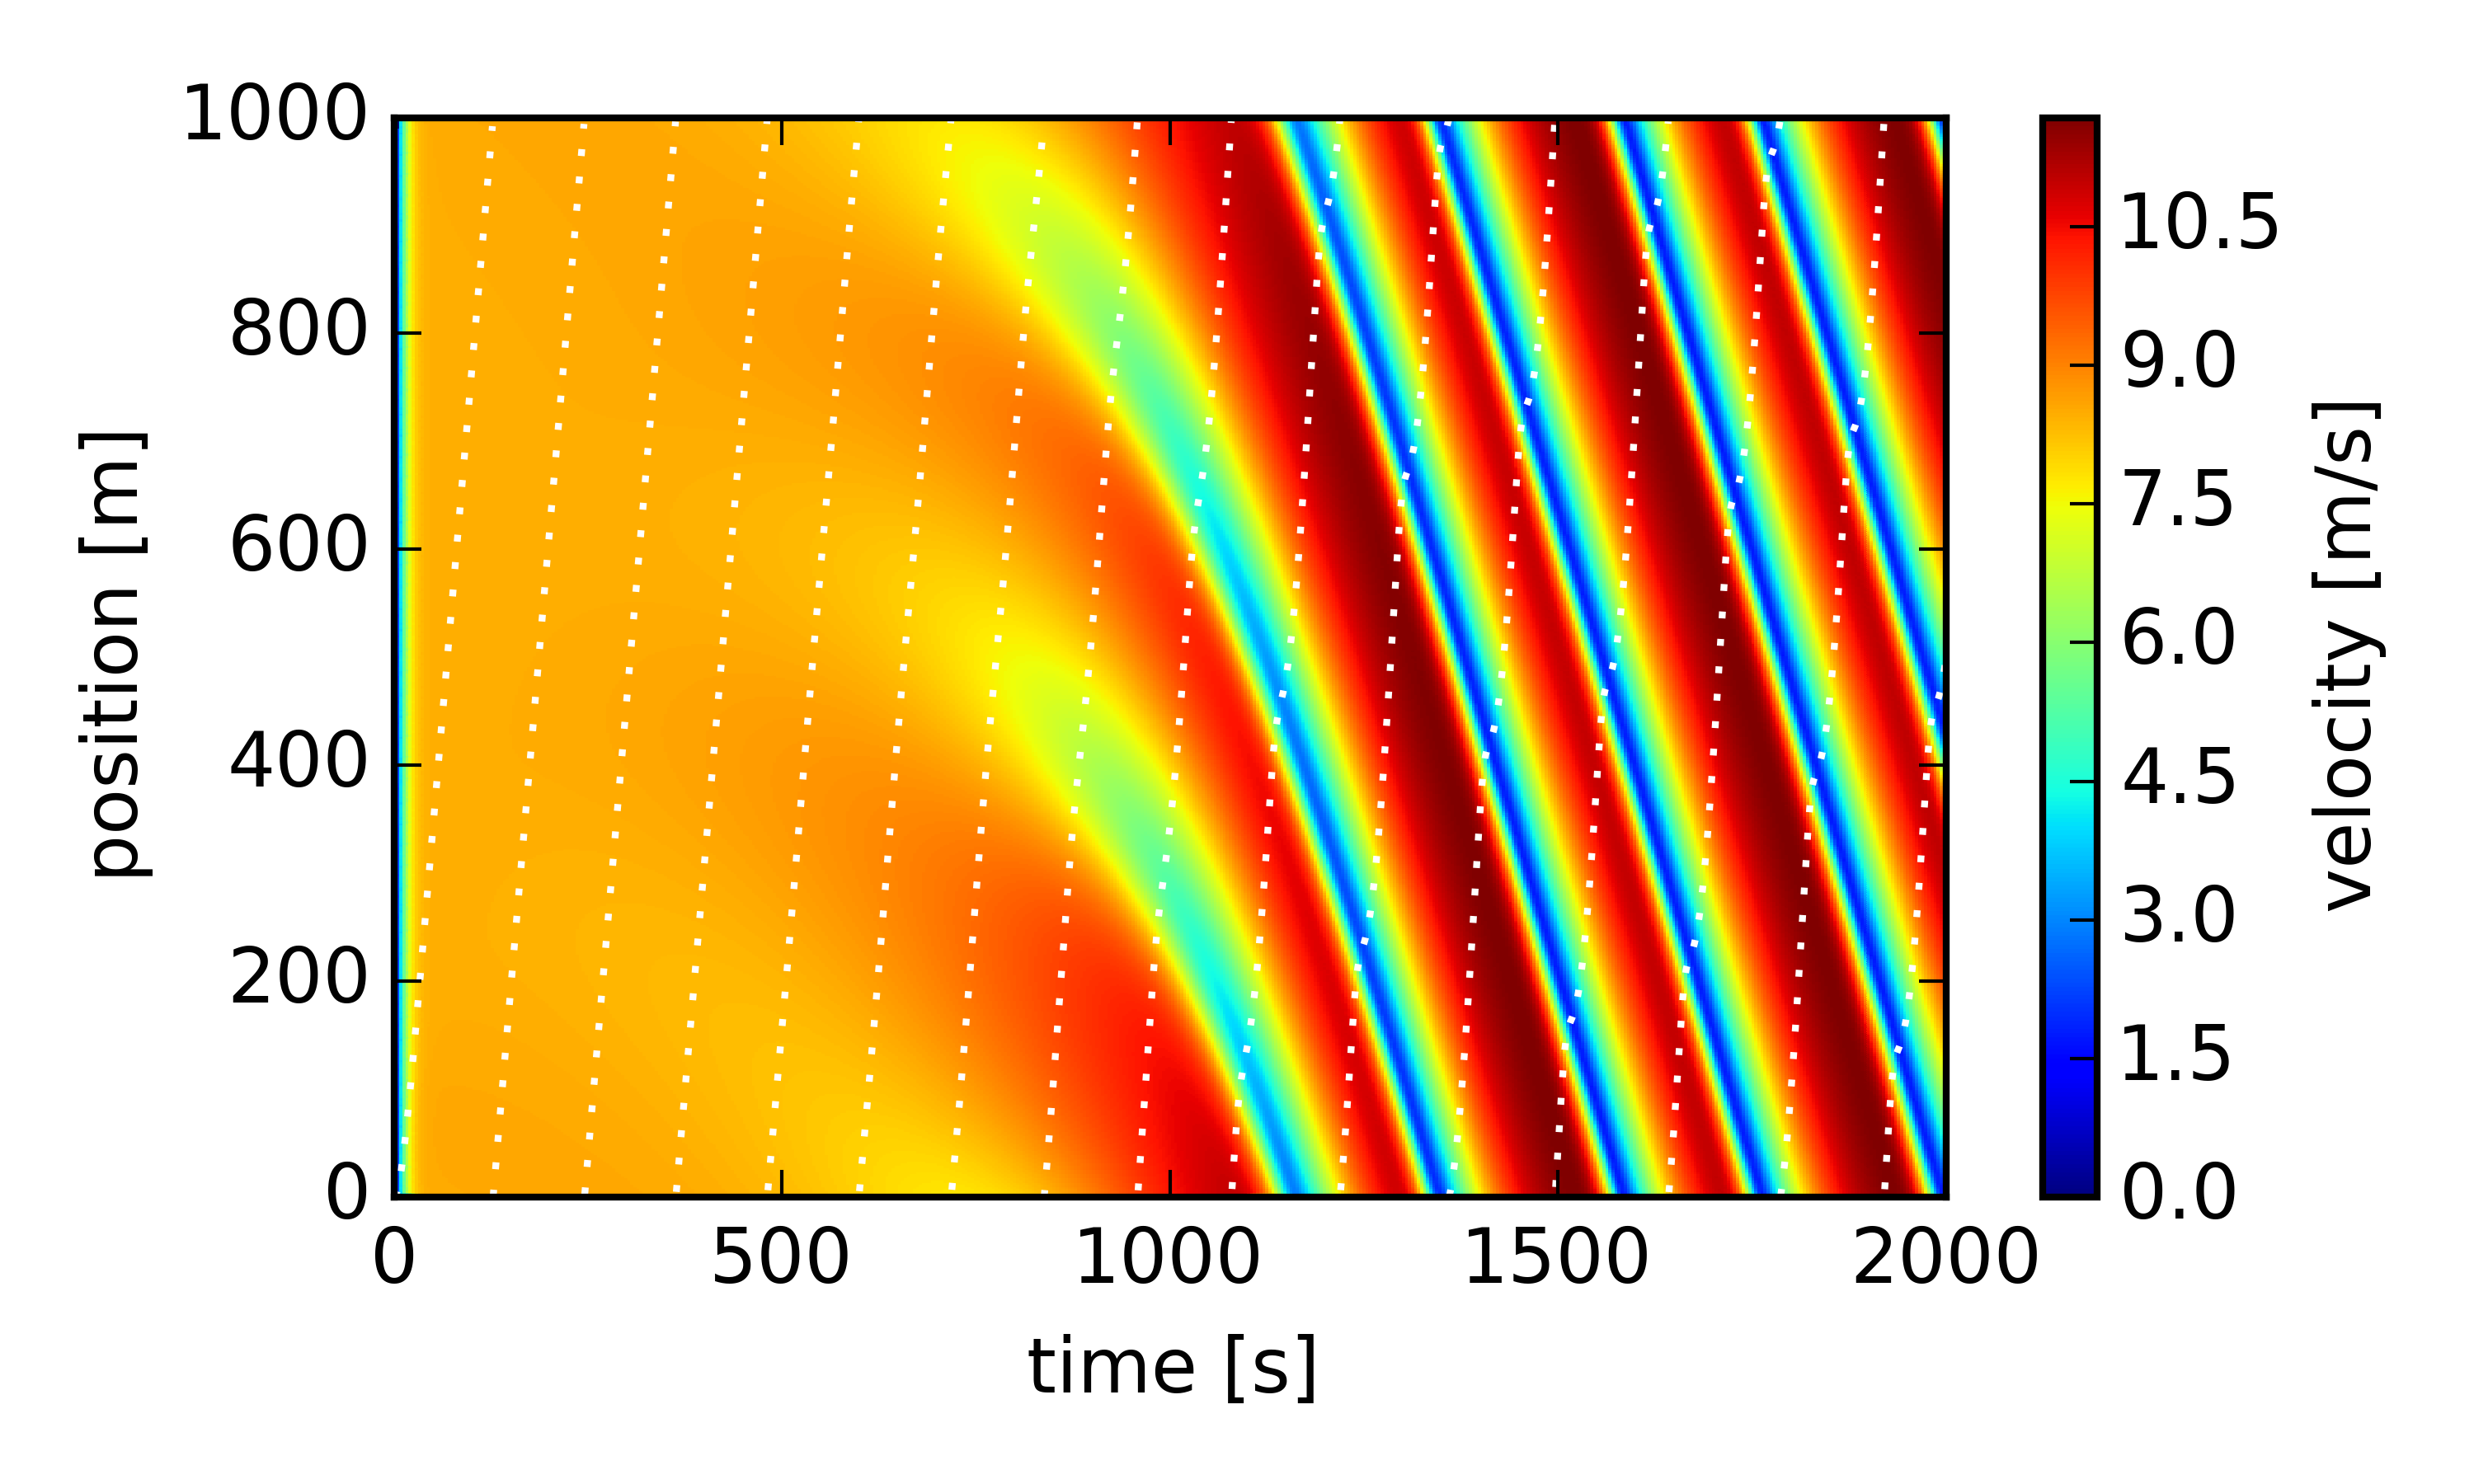
\includegraphics[width=5in]{../img/free_road.png}
    \caption{Spatio-temporal plot of the velocity field with stop-and-go waves. The dotted lines trace the trajectory of a selected car. The $N=50$ vehicles start uniformly distributed along the road. They quickly reach the equilibrium velocity (\SI{\sim 9}{m/s}). After about $t\approx\SI{700}{s}$ the instabilities start to become noticeable, and continue growing until $t\approx \SI{1100}{s}$. Note that the road is assumed to be periodic, hence the stop-and-go-waves, which leave the plot at the bottom, reappear at the top. Also note that the waves travel upstream, i.e. against the flow. For this simulation a time step $\Delta t=\SI{0.125}{s}$ was used.}
    \label{fig:free_road}
\end{figure}
\newpage
\subsection{Instability by asymmetry in acceleration/deceleration behaviour}
\label{sec:asymm}

\begin{wrapfigure}{r}{0.5\textwidth}
    \centering
    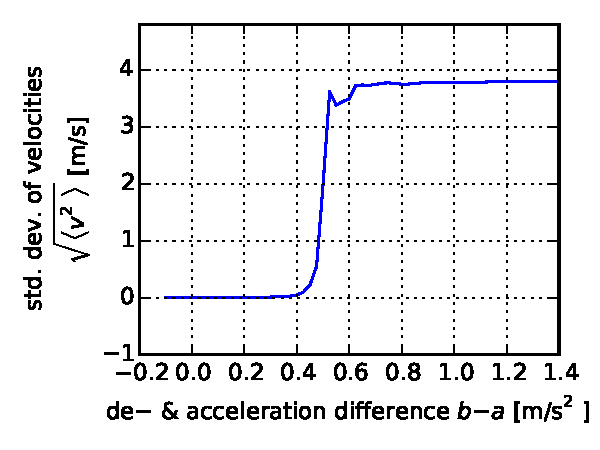
\includegraphics[width=3in]{../img/order_parameter_delta_acceleration.pdf}
    \caption{Instability as a function of the deceleration-acceleration asymmetry. See explanatory text.}
    \label{fig:order_parameter_delta_acceleration}
\end{wrapfigure}
As one can easily imagine, the instabilities are provoked by an asymmetry between the acceleration and deceleration parameters, $a$ and $b$. Indeed, $b$ is typically chosen significantly larger than $a$ (see Table~\ref{tab:param}). A car that is moving particularly slow will not get away fast enough as more cars approach it from behind. The cars stack up, leading to a growing perturbation.

Indeed, when choosing $b$ close to $a$, no instabilities can be observed. In Figure~\ref{fig:order_parameter_delta_acceleration}, the occurrence of instabilities is shown as a function of $b-a$. Clearly, for $b\sim a$ no instabilities are seen, which confirms this conjecture.
For this particular run the acceleration was fixed to $a=\SI{0.6}{m/s^2}$, while $b$ was swept over the according range. The simulation was run for a long time ($t_\mathrm{end} = \SI{500}{min}$). To measure instabilities, the standard deviation of the final velocity distribution was computed. For all further simulations, we use the values for $a$ and $b$ as listed in Table~\ref{tab:param}.

\subsection{Effects of the interaction exponent $\gamma$}
We find that by increasing the exponent $\gamma$, the instabilities vanish as well. All the vehicles' velocity and spacing remain constant and equal to their equilibrium value. The transition from homogeneous traffic to flow prone to instability as a function of $\gamma$ is very sharp. Figure~\ref{fig:order_param} shows this relation. Again the standard deviation of the final velocity distribution was computed as measure for inhomogeneity. As the standard deviation of the velocities vanishes in the homogeneous (disordered) phase, and quickly rises in the inhomogeneous (ordered) phase, it qualifies as an order parameter.

The critical value $\gamma_c$ at which the transition occurs is well defined and mostly independent on the length of the road. Only for $L=\SI{1}{km}$ (blue curve) we see significant finite-size effects.
\begin{figure}
    \centering
    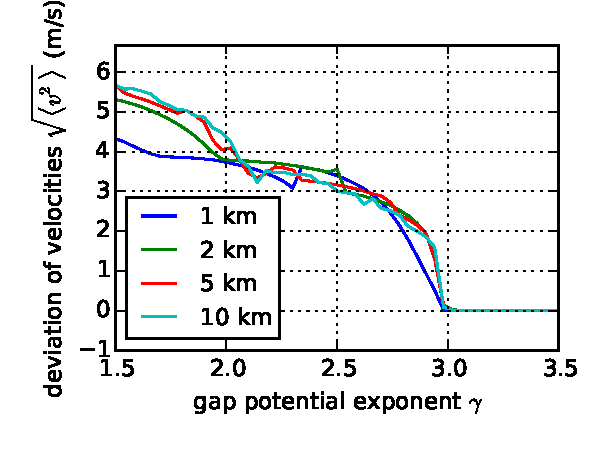
\includegraphics[width=4in]{../img/order_parameter_sweep.pdf}
    \caption{Measure of instabilities as a function of the exponent $\gamma$, for different road lengths. If the traffic remains stable, the velocities are equalized, and hence their variance vanishes. Increasing $\gamma$ beyond a critical value (here $\gamma_c \approx 0.258$) suppresses any instability. The transition appears as a sharp kink in the curve. Although the shape of the curves is slightly different for various road lengths, the critical value $\gamma_c$ is not. For this plot, the vehicle density was fixed to $N/L=\SI{50}{km^{-1}}$.}
    \label{fig:order_param}
\end{figure}

Having established that tuning $\gamma$ gives rise to a sharp transition between phases, it stands to reason to map out this phase boundary as a function of another important parameter. Of particular interest is the density of vehicles, which has also been shown to be responsible for such a phase transition. The result can be seen in Figure~\ref{fig:phase_diagram}. For this the vehicle density was swept, while the corresponding critical exponent $\gamma_c$ was then determined via binary search. It is interesting to note that the phase boundary curve is concave, it reaches a maximum for $N/L \approx \SI{70}{km^{-1}}$. This seems to be the density which is most easily destabilized. Investigating higher vehicle densities than shown in Figure~\ref{fig:phase_diagram} does not bring further insight: as every vehicle requires a space of at least $s_0+l_\alpha= \SI{7}{m}$, the road is completely saturated at $\approx 150$ cars per kilometre. We also find that the shape of the phase boundary is perfectly independent of the length of the road (not shown in this graph).
\begin{figure}
    \centering
    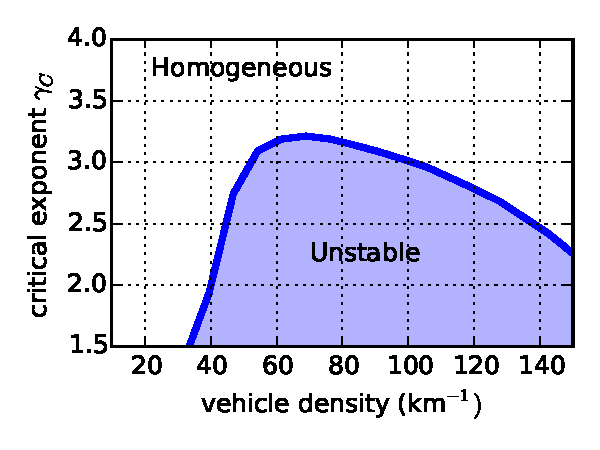
\includegraphics[width=4in]{../img/phase_diagram.pdf}
    \caption{Stability phase diagram with the mean vehicle density on the horizontal axis, and the interaction exponent on the vertical axis. While for the traditional value of $\gamma=2$ the traffic is unstable for a broad range of densities, a higher value of $\gamma$ can render the flow stable at high densities. For the chosen acceleration and deceleration parameters (here $a=\SI{0.6}{m/s^2}$ and $b=\SI{1.5}{m/s^2}$) the flow can be made stable unconditional on the vehicle density.}
    \label{fig:phase_diagram}
\end{figure}


